
% ------------------------------------------------------------------------------
\documentclass[11pt]{report} 
\usepackage{xcolor}
\usepackage{listings}
\definecolor{variablenamecolor}{RGB}{0,0,139}
\usepackage[table,x11names]{xcolor}
\usepackage{projectreport}
\usepackage{longtable}
\usepackage{multirow}
\usepackage{geometry}
\usepackage{float}
\usepackage{colortbl}
\usepackage{hanging}
\usepackage{url}

% ------------------------------------------------------------------------------
% Enter your details here
% ------------------------------------------------------------------------------
\newcommand{\name}{Jorge Rojo}
\newcommand{\course}{CS4097 Independent Research}
\newcommand{\projecttitle}{Cow Pose Estimation}
\newcommand{\submissiondate}{Spring 2024}

% ------------------------------------------------------------------------------
% Document
% ------------------------------------------------------------------------------
\begin{document}

\maketitle

% ------------------------------------------------------------------------------
% Top matter
% ------------------------------------------------------------------------------
\chapter*{Abstract}
The cow pose estimation project aims to develop a computer vision system capable of accurately detecting and estimating the posture of cows in images. Leveraging the YOLO (You Only Look Once) object detection framework and keypoint detection techniques, the project focuses on identifying cows and determining their skeletal keypoints to infer various postures accurately. The dataset used for training and evaluation comprises annotated images of cows, where bounding boxes and landmark keypoints are meticulously labeled. The project involves preprocessing the dataset, training the YOLO model, and fine-tuning it to achieve optimal performance. Additionally, data augmentation techniques are explored to enhance the model's robustness and generalization capabilities. The ultimate goal is to deploy the trained model in real-world scenarios, such as monitoring cattle health and behavior on farms, contributing to advancements in precision livestock farming and animal welfare.



\tableofcontents
% \listoffigures
% \listoftables
%\lstlistoflistings		% comment out if not needed

% ------------------------------------------------------------------------------
% Main matter
% Chapters are added to the document using the \include{chapterx} command
% ------------------------------------------------------------------------------
\newpage
\setcounter{page}{0}
\pagenumbering{arabic}
\chapter{Introduction}
\section{Purpose}
The primary purpose of the cow pose estimation project is to develop a comprehensive and accurate system for monitoring and analyzing the posture and movements of cattle in agricultural settings. By leveraging advanced computer vision techniques, the project aims to address the following key objectives: Enhancing Livestock Welfare, Optimizing Farm Management, Supporting Research and Innovation.
\section{Intended Audience}
This project targets researchers and agricultural scientists engaged in livestock management, as well as professionals in computer vision, machine learning, and artificial intelligence interested in applying their skills to agricultural contexts. Additionally, students and enthusiasts exploring interdisciplinary studies at the intersection of technology and agriculture may find the project's outcomes and methodologies valuable.
\section{Project Scope}
The project encompasses the development and implementation of a cow pose estimation system using deep learning techniques. Key components of the project include data collection and annotation, model training and evaluation, and deployment of the trained model for real-world applications. The scope also extends to exploring data augmentation strategies, optimizing model performance, and assessing the system's accuracy and reliability in diverse agricultural environments. Furthermore, considerations for scalability, usability, and integration with existing livestock management systems will be addressed to ensure the practicality and effectiveness of the proposed solution.
\section{Definitions, Acronyms, \& Conventions}
\begin{table}[h]
    \centering
    \begin{tabular}{|c|p{12cm}|}
        \hline
        \textbf{Term} & \textbf{Definition}\\
        \hline
        YOLO & You Only Look Once\\
        \hline 
        PIL & Python Imaging Library\\
        \hline  
        bbox & Bounding Box\\
        \hline  
        Json & JavaScript Object Notation\\
        \hline  
        Ultralytics & develop and maintain popular tools and libraries, including models for object detection and image classification, such as YOLO (You Only Look Once)\\
        \hline  
        Open-cv &  open-source computer vision and machine learning software library designed to provide a common infrastructure for various applications in the field of computer vision.\\
        \hline  
        
        
    \end{tabular}
\end{table}
% --------------------------------------------------
% Appendices
% --------------------------------------------------
\appendix
\chapter{Phase 1 Backlog}

\section{User Stories}
\begin{longtable}[h!]{|p{1cm}|p{8.6cm}|p{1cm}|p{1.2cm}|p{1.2cm}|p{1.3cm}|}
    \caption*{}
    \centering
    %\begin{tabular}{|p{1cm}|p{11cm}|p{0.8cm}|p{1.2cm}|}
    \hline
    \rowcolor{gray}S. No. & Epic / User Stories & Effort & Priority & Sprint & Owner \\ 
    \midrule
%-------------------------------------------------------------------------------
% Epic 1
%-------------------------------------------------------------------------------
	\rowcolor{lightgray}\textbf{E1}   & \textbf{Research} & \textbf{} & \textbf{High} & \textbf{N/A} & \textbf{N/A}\\
    \hline
    U1.1 & Search for available animal pose datasets online. & &  &  & Jorge\\
    \hline
    U1.2  & Evaluate dataset suitability based on size, annotation quality, and compatibility with YOLO format. &  &  &  & Jorge\\
    \hline
    U1.3  & Explore methods for parsing and preprocessing dataset files.&  &  &  & Jorge\\
    \hline
    \midrule
%-------------------------------------------------------------------------------
% Epic 2
%-------------------------------------------------------------------------------
    \rowcolor{lightgray}\textbf{E2}   & \textbf{Data Collection}   &  \textbf{}  & \textbf{High} & \textbf{N/A} & \textbf{N/A}   \\ 
    \hline
    U2.1 & find suitable data for project & & &&Jorge \\
    \hline
    U2.2 & Pre process raw data &  & & &Jorge \\
    \hline
    U2.3 & Augment dataset for model training &  & &  &Jorge \\
    \hline
   
    
	\midrule
%-------------------------------------------------------------------------------
% Epic 3
%-------------------------------------------------------------------------------
	\rowcolor{lightgray}\textbf{E3}   & \textbf{Model Development} & \textbf{} & \textbf{High} & \textbf{N/A} & \textbf{N/A}\\
    \hline
    U3.1 & YOLO model and configuration &  &  & & Jorge\\
    \hline
    U3.2 & Train the YOLO model &  &  &  &Jorge \\   
    \midrule
 \newpage

%-------------------------------------------------------------------------------
% Epic 4
%-------------------------------------------------------------------------------
    \hline
	\rowcolor{lightgray}\textbf{E4}   & \textbf{Evaluation and Testing} & \textbf{} & \textbf{High} & \textbf{N/A} & \textbf{N/A}\\
    \hline
    U4.1 & Test Model &  &  &  &Jorge \\
    \hline
    U4.2 & Refine Model Parameters &  &  & & Jorge\\

	\midrule

%\end{tabular}
\end{longtable}
\chapter{Implementation}
\newcommand{\key}[1]{\textbf{#1}}
\section{Dataset}
\subsection{Into To Dataset}
\subsubsection{Description}
I discovered a dataset containing animal pose annotations across five categories: dogs, cats, cows, horses, and sheep, encompassing over 6,000 instances distributed across 4,000 images. The annotations for these animals were stored in a JSON format, detailing a total of 20 keypoints. These keypoints include two eyes, throat, nose, withers, two ear bases, tail base, and four each of elbows, knees, and paws. Upon initial inspection, I recognized the potential utility of this dataset. However, to suit my project's requirements, I needed to parse the data and extract only the information relevant to cows.
\newpage
\subsubsection{Describing the original dataset/json}
\begin{lstlisting}[language=Pascal, caption={Original Json Format}, label={lst:}, basicstyle=\ttfamily\scriptsize, frame=single]
    {
        {"images": {"1": "image1.jpg", "2": "image2.jpg",
                            "1999": "image1999.jpg"},.....

        "annotations":
        [{"image_id": 1, 
            "bbox": [123, 115, 379, 275], 
            "keypoints": [[193, 216, 1], [160, 217, 1], [174, 261, 1],
                        [204, 186, 1], [152, 182, 1], [0, 0, 0], 
                            [0, 0, 0], [273, 168, 1], [0, 0, 0], 
                            [0, 0, 0], [0, 0, 0], [266, 225, 1], 
                            [0, 0, 0], [0, 0, 0], [0, 0, 0], 
                            [0, 0, 0], [0, 0, 0], [0, 0, 0], 
                            [190, 145, 1], [351, 238, 1]], 
                            "num_keypoints": 20, 
                            "category_id": 1},...... 
        "categories":
        [{"supercategory": 
            "animal","id": 1, "name": "Dog", 
            "keypoints": ["left_eye", "right_eye", "nose", "left_ear",
                    "right_ear", "left_front_elbow",
                    "right_front_elbow", "left_back_elbow", "right_back_elbow",
                    "left_front_knee", "right_front_knee", "left_back_knee", 
                    "right_back_knee", "left_front_paw", "right_front_paw", 
                    "left_back_paw", "right_back_paw", "throat", "withers", "tailbase"], 
            "skeleton": [[0, 1], [0, 2], [1, 2], [0, 3], [1, 4], [2, 17], 
            [18, 19], [5, 9], [6, 10], [7, 11], [8, 12], [9, 13], [10, 14], 
            [11, 15], [12, 16]]},....
    }
\end{lstlisting}
\newpage
The "\key{images}" field contains a dictionary where each key represents the image identifier, and its corresponding value is the filename of the image.\newline
The "\key{annotations}" field contains a list of dictionaries, each representing an annotation entry for an image. Each annotation dictionary includes the following fields:
\begin{itemize}
    \item "\key{image\_id}": An identifier for the image to which this annotation corresponds.
    \item "\key{bbox}": A list representing the bounding box coordinates of the annotated object in the format (x\_min, y\_min, width,height).
    \item "\key{keypoints}": A list of lists representing the keypoint coordinates for the annotated object. Each keypoint is represented as [x\_coordinate, y\_coordinate, visibility], where visibility indicates whether the keypoint is visible (1) or not (0).
    \item "\key{num\_keypoints}": The total number of keypoints annotated for the object.
    \item "\key{category\_id}": The category identifier of the annotated object.
\end{itemize}
The "\key{categories}" field contains information about the categories of annotated objects. Each category entry is represented as a dictionary with the following fields:
\begin{itemize}
    \item "\key{supercategory}": The supercategory to which the category belongs.
    \item "\key{id}": The unique identifier for the category.
    \item "\key{name}": The name of the category.
    \item "\key{keypoints}": A list of keypoint names associated with the category.
    \item "\key{skeleton}": A list representing the skeletal connections between keypoints for visualization purposes.
\end{itemize}
Though this dataset provides detailed annotations for various animal categories. The first plan was to restructure the dataset
\newpage
\subsubsection{Data Preparation}
Since I adopted the approach of reference learning, several adjustments were necessary:

1. Initially, I parsed the JSON dataset and extracted only the cow-related information. This involved filtering the annotations to include entries corresponding to category 5 (cows). The filtered annotations were then stored in a new list of dictionaries. Additionally, I parsed the image folder to select only the images associated with the filtered annotations.
\textit{"This greatly reduced my amount of data from 4000 images to around 500"}

2. Subsequently, I restructured the JSON data to ensure that each entry in my dictionary contained all the relevant information for a cow.

3. However, I realized that important metadata, such as the height and width of the images, was missing. To rectify this, I utilized the Python Imaging Library (PIL) to extract the dimensions of each image.

4. With all the necessary information at hand, I proceeded to research the formatting requirements of YOLO for Pose estimation.
\newline
\newline
\newline
\newline
\newline
\newline
\newline
\newline
\newline
\newline
\newline
\newline
\newline
\newline
On the next page i have provided the structure of the new JSON as well as describing the code and its format
\newpage
\begin{lstlisting}[language=Pascal, caption={New Json Format}, label={lst:}, basicstyle=\ttfamily\scriptsize, frame=single]
{
    "img_path": "image1.jpg",
    "img_width": 375,
    "img_height": 500,
    "img_boxes": [[x_min, y_min, width, height]],
    "img_joints": [
        [x1, y1, v1], [x2, y2, v2], ..., [x19, y19, v19]
    ]
},
{
    "img_path": "image2.jpg",
    "img_width": 400,
    "img_height": 600,
    "img_boxes": [[x_min, y_min, width, height]],
    "img_joints": [
        [x1, y1, v1], [x2, y2, v2], ..., [x19, y19, v19]
    ]
},
...
\end{lstlisting}
\begin{itemize}
    \item \textbf{img\_path}: The file path of the image.
    \item \textbf{img\_width}: The width of the image in pixels.
    \item \textbf{img\_height}: The height of the image in pixels.
    \item \textbf{img\_boxes}: A list of bounding boxes representing the annotated object in the format \texttt{[x\_min, y\_min, width, height]}. These values are normalized relative to the image dimensions, where \texttt{x\_min} and \texttt{y\_min} represent the coordinates of the top-left corner of the bounding box, and \texttt{width} and \texttt{height} represent the dimensions of the bounding box.
    \item \textbf{img\_joints}: A list of keypoint coordinates for the annotated object. Each keypoint is represented as \texttt{[x, y, visibility]}, where \texttt{x} and \texttt{y} are the coordinates of the keypoint normalized to the range [0, 1] relative to the image dimensions, and \texttt{visibility} indicates whether the keypoint is visible (1) or not (0).
\end{itemize}
\newpage


\section{Data Preprocessing for YOLO Training}
\subsection{Ultralytics YOLO Format}
After obtaining the required image and annotation data. I conducted more researched to understand the specific formatting required for YOLO (You Only Look Once) object detection models. This led to me discovering that YOLO expects bounding box coordinates and associated keypoint annotations in a particular text-based format for training. Below I have displayed the documentation on ULTRALYTICS documentation.

\begin{itemize}
    \item One text file per image: Each image in the dataset has a corresponding text file with the same name as the image file and the ".txt" extension.
    \item One row per object: Each row in the text file corresponds to one object instance in the image.
    \item Object information per row: Each row contains the following information about the object instance:
    \begin{itemize}
        \item Object class index: An integer representing the class of the object (e.g., 0 for person, 1 for car, etc.).
        \item Object center coordinates: The \(x\) and \(y\) coordinates of the center of the object, normalized to be between 0 and 1.
        \item Object width and height: The width and height of the object, normalized to be between 0 and 1.
        \item Object keypoint coordinates: The keypoints of the object, normalized to be between 0 and 1.
    \end{itemize}
\end{itemize}
\textit{"This section outlines the dataset label format for training YOLO pose models, adapted from the Ultralytics documentation."}

\newpage
\subsection{Conversion Method}
\begin{lstlisting}[language=Pascal, caption={YOLO Formatting Fucntions}, label={lst:}, basicstyle=\ttfamily\scriptsize, frame=single]
def create_yolo_boxes_kpts(img_size, boxes, lm_kpts):
    IMG_W, IMG_H = img_size
    norm_bbox_per_img = boxes / np.array([IMG_W, IMG_H, IMG_W, IMG_H])
    norm_kps_per_img = lm_kpts.copy()
    norm_kps_per_img[:, :, :-1] /= np.array([IMG_W, IMG_H])
    yolo_data = []
    for i in range(len(boxes)):
        yolo_data.append("0")  # Class Label
        # Bounding Box Coordinates
        bbox = norm_bbox_per_img[i]
        yolo_data.append(f" {bbox[0]:.6f} {bbox[1]:.6f} {bbox[2]:.6f} {bbox[3]:.6f}")
        for kpt in norm_kps_per_img[i]:
            for coord in kpt[:-1]:
                yolo_data.append(f" {coord:.6f}")
            visibility = "2" if kpt[-1] != 0 else "0"
            yolo_data.append(f" {visibility}")
        if i < len(boxes) - 1:
            yolo_data.append("\n")
    return "".join(yolo_data)
def create_yolo_txt_files(json_data, LABEL_PATH):
    for data in json_data:
        IMAGE_ID = data["img_path"].split("/")[-1].split(".")[0]
        IMG_WIDTH, IMG_HEIGHT = data["img_width"], data["img_height"]
        landmark_kpts = np.nan_to_num(np.array(data["img_joints"], dtype=np.float32))
        landmarks_bboxes = np.array(data["img_boxes"], dtype=np.float32)
        yolo_data = create_yolo_boxes_kpts((IMG_WIDTH, IMG_HEIGHT), landmarks_bboxes,
        landmark_kpts)
        TXT_FILE = IMAGE_ID + ".txt"
        with open(os.path.join(LABEL_PATH, TXT_FILE), "w") as f:
            f.write(yolo_data)
create_yolo_txt_files(train_json_data, TRAIN_LABEL_PATH)
create_yolo_txt_files(val_json_data, VALID_LABEL_PATH)
\end{lstlisting}
These functions collectively convert the collected image and annotation data into the required YOLO format, facilitating the training of object detection models.
\newpage
\subsection{Text Files}
\begin{lstlisting}[language=Pascal, caption={Txt File Format}, label={lst:}, basicstyle=\ttfamily\scriptsize, frame=single]
0 0.556000 0.274667 0.698000 0.392000 0.000000 0.000000 0 0.686000 ..........
0 0.442000 0.282667 0.564000 0.394667 0.000000 0.000000 0 0.000000 .........
0 0.268000 0.274667 0.446000 0.394667 0.000000 0.000000 0 0.426000 .......
0 0.196000 0.258667 0.288000 0.354667 0.228000 0.290667 2 0.214000 ..........
\end{lstlisting}
The snippet above is a text file for an image containing 4 "objects/cows" each entry being on a newline
\newline
\newline
\newline
\newline
\begin{figure}[htbp]
    \centering
    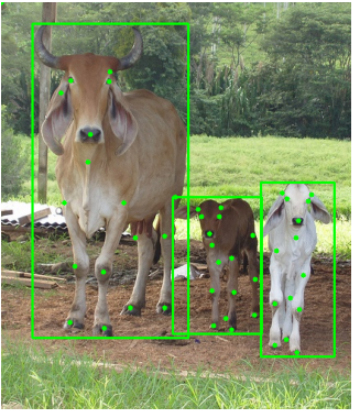
\includegraphics[width=.5\textwidth]{Images/annotation.png}
    \caption{Training results.}
    \label{fig:trainresults}
\end{figure}

\textit{    "This is an image visualized with the an image and its corresponding text file."}
\newpage
\section{Training the Model}

After an initial training run of just one epoch to ensure that all parameters were properly configured, the model underwent a more extensive training phase consisting of 60 epochs. Monitoring the training progress through various performance metrics, it became apparent that the model's accuracy plateaued around epochs 45 to 55, showing no significant improvement thereafter. Despite the extended training period, the resulting performance metrics were disappointing, prompting a closer examination of the data used for training. This analysis revealed underlying issues within the dataset itself, suggesting that the observed limitations in model performance were not solely attributed to the duration of training, but rather to the quality or amount of the training data.
\newline
\begin{figure}[htbp]
    \centering
    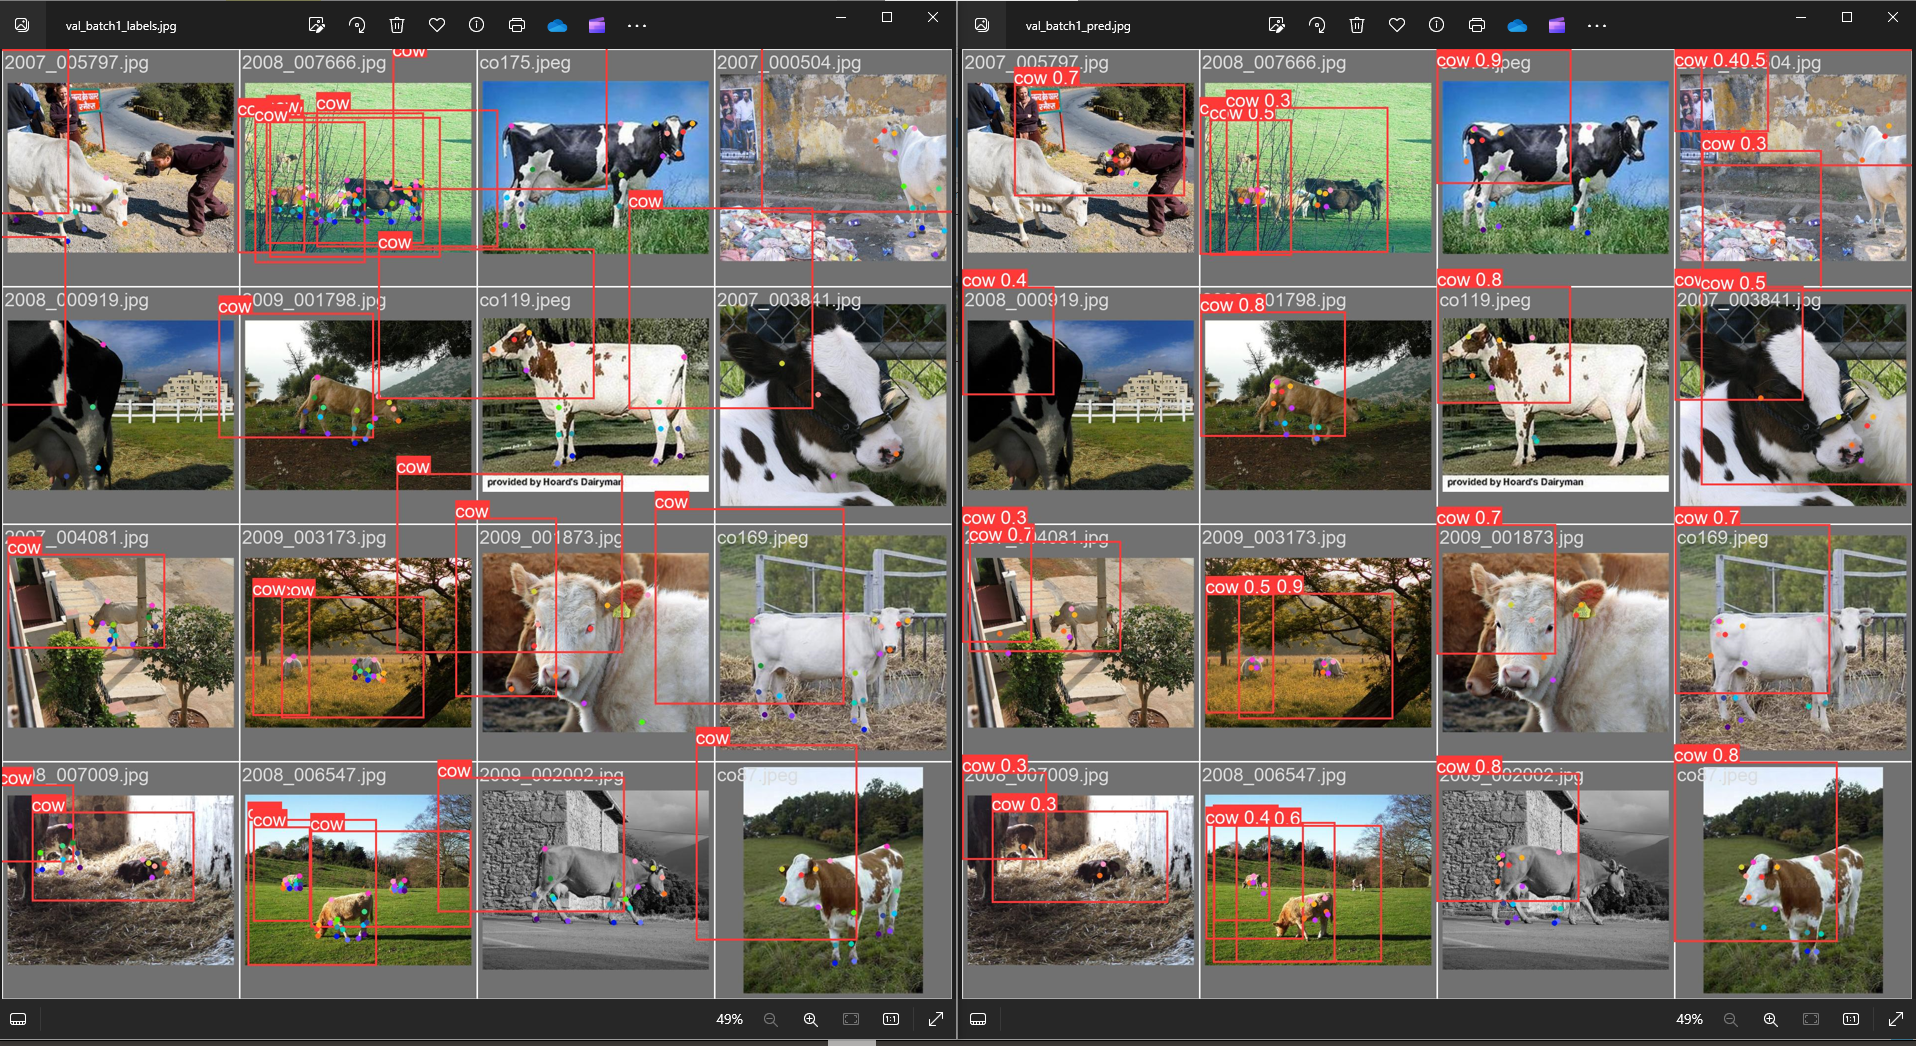
\includegraphics[width=1.05\textwidth]{Images/trianresults.png}
    \caption{Training results.}
    \label{fig:trainresults}
\end{figure}

\begin{figure}[htbp]
    \centering
    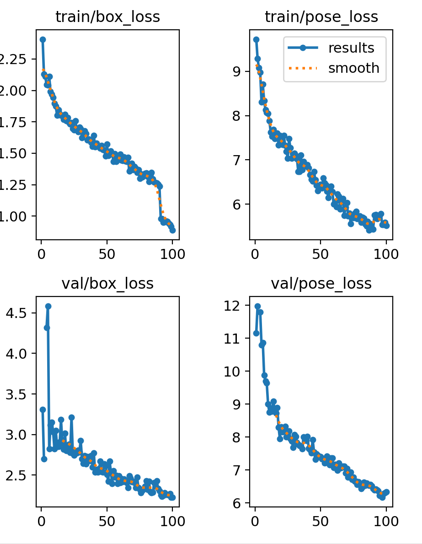
\includegraphics[width=.8\textwidth]{Images/trainposeloss.png}
    \caption{Training results.}
    \label{fig:trainresults}
\end{figure}
\newpage
\section{Improving the model}
Now that it has become apparent that the lack of data is a significant factor contributing to the subpar accuracy of the model, efforts will be focused on augmenting the existing dataset to improve its diversity. Data augmentation techniques will be employed to generate additional training examples. This will involve operations such as rotating the images and their corresponding coordinates to introduce variations in orientation. Additionally, flipping or reflecting the images along with their coordinates will be explored to further improve the dataset. 

\chapter{References}
\begin{hangparas}{4em}{1} % 1em hanging indent, 1 line of hanging
Dataset Reference:\newline
Title: Cross-Domain Adaptation for Animal Pose Estimation\newline
Authors: Jinkun Cao, Hongyang Tang, Hao-Shu Fang, Xiaoyong Shen, Cewu Lu, Yu-Wing Tai\newline
Publication Venue: The IEEE International Conference on Computer Vision (ICCV)\newline
Year: 2019
\newline
Citation Format: [@InProceedings{Cao_2019_ICCV}]\newline
URL: [https://sites.google.com/view/animal-pose/]
\end{hangparas}
\newline
\newline
\begin{hangparas}{4em}{1} % 1em hanging indent, 1 line of hanging
    URL:[https://docs.ultralytics.com/datasets/pose/#supported-dataset-formats]
\end{hangparas}
\newline
\newline
\begin{hangparas}{4em}{1} % 1em hanging indent, 1 line of hanging
Unlocking Animal Pose Estimation with YOLOv8: Fine-tuning for Dogs\newline
URL[https://www.youtube.com/watch?v=kb03ufEkOdA&t=240s]
\end{hangparas}

\begin{hangparas}{4em}{1} % 1em hanging indent, 1 line of hanging
DeepLabCut: a software package for animal pose estimation\newline
URL[https://github.com/DeepLabCut/DeepLabCut]
\end{hangparas}

\begin{hangparas}{4em}{1} % 1em hanging indent, 1 line of hanging
Deep learning pose estimation for multi-cattle lameness detection\newline 
URL[https://www.nature.com/articles/s41598-023-31297-1]
\end{hangparas}

\begin{hangparas}{4em}{1} % 1em hanging indent, 1 line of hanging
Precision livestock farming for pigs\newline 
URL[https://academic.oup.com/af/article/7/1/32/4638771]
\end{hangparas}

\begin{hangparas}{4em}{1} % 1em hanging indent, 1 line of hanging
An intelligent system for livestock disease surveillance\newline 
URL[https://www.sciencedirect.com/science/article/abs/pii/S0020025516312658]
\end{hangparas}
\chapter{Summary \& Future Work}
\section{Research Efforts}
The majority of the project's time was dedicated to research, particularly due to the novelty of the topic and its complexities. As a newcomer to the field of pose estimation, extensive time was spent on understanding the underlying principles, exploring relevant literature, and familiarizing myself with computer vision and machine learning. 

Additionally, quite some time was invested in investigating available datasets, and understanding data preprocessing techniques.

Moving forward, the knowledge acquired during this research phase will not only help immensely to continue and shape the project's trajectory but also with anything related to pose estimation and computer vision.
\section{Overall}
Throughout the project duration,  Significant progress has been made in the research and learning of pose estimation, ultralytics, and computer vision. Leveraging cutting-edge techniques in computer vision and machine learning, we have developed a system capable of identifying and tracking key anatomical landmarks on cows. Despite encountering challenges, such as data preprocessing complexities and model optimization intricacies, the project has successfully implemented core functionalities for accurate cow pose estimation.

However, it's important to note that the model still does not consistently yield accurate results. Moving forward, the next step would involve data augmentation techniques to enhance the model's performance. These techniques, such as rotating images and their corresponding coordinates, flipping or reflecting images, and augmenting the dataset, have the potential to improve the model's accuracy and generalization capabilities.

Regrettably, due to time constraints, further exploration and refinement of these techniques must be postponed. Nonetheless, these plans remain on the agenda for future iterations of the project. With additional time and resources, the project can continue to evolve, paving the way for more accurate and reliable cow pose estimation systems in the agricultural domain.




% ------------------------------------------------------------------------------
% Reference list
% ------------------------------------------------------------------------------
\addcontentsline{toc}{chapter}{References}
\renewcommand\bibname{References}
\printbibliography

% ------------------------------------------------------------------------------
% Appendices
% ------------------------------------------------------------------------------
% \include{appendix}

\end{document}